%%%%%%%%%%%%%%%%%%%%%%%%%%%%%%%%%%%%%%%%%%%%%%%%%%%%%%%%%%%%%%%%%%%%%%%%
\chapter[The Rural Household Multi-Indicator Survey for rapid characterisation of rural households]{The Rural Household Multi-Indicator Survey for rapid characterisation of rural households}
%%%%%%%%%%%%%%%%%%%%%%%%%%%%%%%%%%%%%%%%%%%%%%%%%%%%%%%%%%%%%%%%%%%%%%%%
\chaptermark{The Rural Household Multi-Indicator Survey}
\label{cha:chapter2}
\vspace*{\fill}
This chapter is based on:
\\
\\
% Full citation of the published (or submitted/in review) article
% This refers to the article key in the refs.bib file.
%\bibentry{Hammond2017225}
Hammond, J., Fraval, S., van Etten, J., Suchini, J. G., Mercado, L., Pagella, T., Frelat, R., Lannerstan, M., Douxchamps, D., Teufel, N., Valbuena, D., van Wijk, M. T. (2017). The Rural Household Multi-Indicator Survey (RHoMIS) for rapid characterisation of households to inform climate smart agriculture interventions: Description and applications in East Africa and Central America. \textit{Agricultural Systems, 151}, 225–233. doi:10.1016/j.agsy.2016.05.003
\\
\\
A full version of the RHOMIS tool is available in \citealp[pp.~114-131]{Hammond2018}. Refer to the following weblink \href{https://research.bangor.ac.uk/portal/files/22079255/2018_Hammond_J_PhD.pdf#page=132}{link}: \url{https://research.bangor.ac.uk/portal/files/22079255/2018_Hammond_J_PhD.pdf#page=132}
\newpage

%%%%%%%%%%%%%%%%%%%%%%%%%%%%%%%%%%%%%%%%%%%%%%%%%%%%%%%%%%%%%%%%%%%%%%%%
\section{Abstract}
%%%%%%%%%%%%%%%%%%%%%%%%%%%%%%%%%%%%%%%%%%%%%%%%%%%%%%%%%%%%%%%%%%%%%%%%
The rural household multi-indicator survey (RHOMIS) is designed to rapidly characterise a series of standardised indicators of agricultural production and market integration, nutrition, food security, poverty and GHG emissions. The core of the survey takes 40–60 min to administer per household using a digital implementation platform. This is linked to a set of automated analysis procedures that enable immediate cross-site bench-marking and intra-site  characterisation. We trialled the survey in two contrasting agro-ecosystems, in Lushoto district of Tanzania (n = 150) and in the Trifinio border region of Guatemala, El Salvador and Honduras (n = 285). The tool rapidly characterised variability between farming systems at landscape scales in both locations identifying key differences across the population of farm households.




\newpage



%%%%%%%%%%%%%%%%%%%%%%%%%%%%%%%%%%%%%%%%%%%%%%%%%%%%%%%%%%%%%%%%%%%%%%%%
\section{Introduction}
%%%%%%%%%%%%%%%%%%%%%%%%%%%%%%%%%%%%%%%%%%%%%%%%%%%%%%%%%%%%%%%%%%%%%%%%

At present, approximately 75\% of the world's poor live in rural areas (\citealp{Livingston2011}), and many of those are in areas where climate change is expected to have a significant detrimental impact on top of current and future agricultural demand and development challenges.

Predicted changes in rainfall and temperature patterns will strongly affect agricultural production, with changed crop production and yields; causing increased vulnerability of many rural communities. As much as 22\% of the cultivated area under the world's most important crops is projected to experience negative impacts from climate change by 2050, with as much as 56\% of the land area in sub-Saharan Africa being impacted (\citealp{Campbell2011}). The overall aim of Climate smart agriculture (CSA) is to `support efforts from the local to global levels for sustainably using agricultural systems to achieve food and nutrition security for all people at all times, integrating necessary adaptation and capturing potential mitigation' (\citealp{Lipper20141068}; \citealp{Neufeldt2013}). Climate smart agriculture therefore has three main pillars, to be considered at different spatial and temporal scales (\citealp{FAO2013570}): 1) achieve food security, 2) adapt and build resilience to climate change and 3) reduce greenhouse gas emissions to mitigate further climate change.

There is an urgent need to improve the characterisation of agricultural systems at household level to enable a more efficient assessment of the capacity households to adopt of climate smart measures. Capacity to adopt is intrinsically linked with the potential success of those measures, which means assessing trade-offs amongst multiple outcome objectives for adopters. Local drivers and factors need to be identified that might constrain or provide opportunities within a specified agricultural system (\citealp{Carletto2015133}), while on the other hand generalisable standardised characteristics need to be identified that would allow robust comparisons between different systems (\citealp{Frelat2016458}; \citealp{vanWijk201477}).

One way to assist the assessment of opportunities at smallholder farm household level for CSA can be through integration of standardised agricultural, poverty, nutrition and environmental indicators in the quantitative characterisation of these households. This will allow us to assess how these performance indicators vary across a farm population, across different sets of farm practices present in the farm population and across different agro-ecological and socio-economic conditions as well as how they may change over time. At present household level characterisation studies are hampered by a variety of problems. A recent analysis of farm household level survey data collected in different agricultural development oriented projects, showed large differences in content between different survey instruments, with lack of standardisation of indicators and evidence that only a small amount of the information collected during lengthy surveys could actually be used for cross-site comparisons (\citealp{Frelat2016458}). This lack of standardisation in combination with often relatively poor data quality (\citealp{Tiffen2003}), generally caused by unsuitable survey design (\citealp{Randall2015162}) or by biases due to perverse incentives (\citealp{Sandefur2015116}), has led to a lack of quantitative insight beyond the locality of each study regarding the effect of interactions between proposed adaptation options and the wider socio-economic and biophysical environment on household level performance indicators. For example, we know little on how household food security has been affected by trends in agricultural production in different regions of the world (\citealp{Carletto2013}) or what the effects of adopting CSA measures are. The lack of integrated survey approaches hampers our knowledge of trade-offs and/or synergies between indicators at farm household level (e.g. \citealp{Klapwijk2014110}). Furthermore, it is unknown how these relationships and trade-offs are shaped by farm management and by social and bio-physical environments (\citealp{Carletto2015133}; \citealp{DeWeerdt201536}).

In this paper we describe a new standardised modular survey tool called rural household multi-indicator survey (RHOMIS) that tries to overcome the current problems associated with household characterisation surveys. The RHOMIS tool is constructed from a set of
standardised performance indicators that run across the three pillars of CSA, and aims to allow us to quantitatively analyse the links between agricultural management strategies and farm household performance.


%%%%%%%%%%%%%%%%%%%%%%%%%%%%%%%%%%%%%%%%%%%%%%%%%%%%%%%%%%%%%%%%%%%%%%%%
\section{Methods}
%%%%%%%%%%%%%%%%%%%%%%%%%%%%%%%%%%%%%%%%%%%%%%%%%%%%%%%%%%%%%%%%%%%%%%%%

%%%%%%%%%%%%%%%%%%%%%%%%%%%%%%%%%%%%%%%%%%%%%%%%%%%%%%%%%%%%%%%%%%%%%%%%
\subsection{Principles and general design of the RHOMIS tool}

The RHOMIS (Rural Household Multiple Indicator Survey) tool consists of a farm household survey that can be conducted on a digital platform using smart phones or tablets using the open data kit (ODK) suite  of software installed on Android based mobile phones or tablets (\citealp{Hartung2010}). Data can be directly uploaded to a web-server, and an associated set of analysis tools programmed in R extract the data and calculate indicators. The tool has been set up in such a way that additional modules of questions and indicators can be incorporated and analysed depending on the local study needs. The survey tool was designed according to the following five principles:
\begin{enumerate}[label=\roman*.]
\item the survey has to be rapid enough to avoid participant fatigue or annoyance, and keeping costs low to allow for larger sample sizes on a limited budget;
\item the survey has to be utilitarian, in that all questions asked in the survey are being used in pre-defined analyses, in order to minimise superfluous data collection;
\item the survey has to be user-friendly, so that all participants in the process of collecting and analysing data can perform the tasks with minimum hassle and resistance, and therefore increase speed and data quality;
\item the survey has to be flexible, so that it can be modified easily to suit the local context of the farming systems and farm households where it will be deployed;
\item the data gathered has to be reliable, in that questions should be easy for respondents to understand and the answers should be based on observable criteria or respondents' direct experience rather than abstract scales or abstract concepts.
\end{enumerate}

\subsection{Household performance indicators}

The indicators that are captured by the RHOMIS tool were chosen to represent important factors of the agricultural production, nutrition and poverty, while also capturing key indicators of interest related to CSA (i.e. greenhouse gas emissions and gender equity). The survey tool was constructed in a modular way, with each module collecting the information needed to be able to calculate the performance indicator of interest. New indicators of interest to the user can therefore be added easily. The indicator set collected in the initial version of the RHOMIS tool consisted of the following elements:

\begin{enumerate}[label=\arabic*., start = 1]
\item Food availability is supply-based estimate of the potential amount of food that can be generated through on and off-farm activities by any one household, and is measured in kilo-calories (kcal) per person (adult equivalent) per day (\citealp{Frelat2016458}; \citealp{Ritzema2017}; \citealp{VanWijk2014a}). The indicator is calculated from on-farm consumption of food crops and livestock products, and from the amount of food (local staple crop) that could be purchased using the cash incomes earned through selling farm produce and through off-farm activities. It ignores farm costs and household expenses, and therefore only gives an indication of whether certain activities lead to enough food being potentially available to feed the family, and the relative importance of these activities compared to each other. It does not quantify actual consumption.
\item The household dietary diversity score (HDDS) is calculated according to the number of different food groups consumed over a given reference period, and is a proxy indicator for diet diversity, the improvement of which is associated with a number of key health indicators such as birth weight, child anthropometric status, and improved haemoglobin concentrations. The HDDS score in RHOMIS follows the instructions of \citet{Swindale2006} in most aspects but departs from the standard advice in terms of reference time period. A 24 h recall method is recommended, but we instead asked how often foodstuffs from each food group were eaten during a 4 week period in `the flush period' and `the lean period'; where respondents could answer that they consume foods from each group either `daily', `weekly', `monthly', or `never/less then monthly'. Whilst this approach might result in lower accuracy than a 24 h recall, the required survey intensity is much less in order to capture seasonal variations. The 12 food groups used were standard, but locally appropriate examples were chosen in each location. The indicator results are on a scale of 0 to 12, where 12 is the most diverse diet in which all 12 food groups are eaten on at least a weekly basis. The data on consumption frequency within the recall period will allow us more complex interpretations in terms of micro-nutrient use, but will not be analysed in this study.
\item The Household Food Insecurity Access Scale (HFIAS) indicator estimates the prevalence of food insecurity and is based on the idea that the experience of food insecurity (access to food) causes predictable reactions and responses that can be captured and quantified through a survey and summarised in a scale. There are nine questions that represent a generally increasing level of severity of food insecurity, and nine “frequency-of-occurrence” questions that are asked as a follow-up to each occurrence question to determine how often the condition occurred (\citealp{Coates2007}). The approach has been applied successfully in numerous studies in developing countries (\citealp{Coates2006}). We asked respondents about food insecurity during the worst month (`lean period') of the previous year, and frequency options were again `daily',
weekly', `monthly',or `never/less then monthly'. The indicator is scored on a range of 0 to 27, where a higher number means a household experiences more food insecurity.
\item The Progress out of Poverty Index (PPI) is a widely used standard indicator of poverty (\citealp{Desiere201510}). The PPI is a rapid ten-question survey which estimates the likelihood that a household has an expenditure below a given poverty line, where the score ranges between 0 and 100, and a higher score means a household is less likely to be below the poverty line (\citealp{GrameenFoundation2015}). The scorecard uses ten simple indicator questions based on observable household characteristics that are correlated with poverty levels using Living Standards Measurement Surveys or similar, detailed surveys. The PPI approach is now available for 55 countries, amongst which are Guatemala and Tanzania.
\item A gender equity indicator was included to quantify the role of women in decision-making and household resource management. The inclusion of gender in resilience and vulnerability assessments is a burgeoning topic (\citealp{Smyth2015405}; \citealp{Morchain2015481}), and achieving gender equity is an aim of many policies in developing countries. The indicator is constructed based on three questions asked for each farm product or income source: who does most of the work, who usually decides when to eat it, and who sells it; where the possible answers are `household males', `household females' and/or `children'. The information was aggregated to an overall score by weighing each activity along the importance it has in the food availability indicator, resulting in a final score between 0 and 1, where 1 implies that female decides completely what happens with the benefits generated by different on and off farm activities. This indicator therefore does not deal with ownership of resources, but with the agency to decide what to do with the benefits that result from these resources. We constructed a novel indicator in this case, because although alternatives do exist, they were too detailed and complex for our purposes (\citealp{Johnson2015}). For example, the Women's Agricultural Empowerment Index requires 60– 80 minutes of interview time per household (\citealp{Alkire2013}), which is longer than our target time for the full questionnaire.

\item Farm level estimates of greenhouse gas (GHG) emissions were calculated using the IPCC Tier 1 approach (\citealp{IPCC2006}). Tier 1 was chosen because it is a recognised method and has low data demands. Although the Tier 2 approach yields a more detailed GHG assessment, the substantially higher data demands can lead to unreliable data when relying on farmer recall. Key determinants of the Tier 1 estimate of emissions for this indicator are number of cattle and other livestock, land use area and type, inputs of mineral fertiliser and the production and use of manure and crop residues. The indicator does not account for carbon sinks, land use change (even if implemented longitudinally), capital infrastructure,
\end{enumerate}
\begin{enumerate}[label=\arabic*., start=6]
\item nor farm related electricity or fuel use. Farm greenhouse gas emissions are reported in kilograms CO2-equivalent per farm per year.
\end{enumerate}

These were the six core indicators that can be quantified with this version of the RHOMIS tool. The information used to calculate these indicators was also used to calculate several other performance indicators:
The questions used to calculate the Food Availability indicator were used to quantify
\begin{enumerate}[label=\arabic*., start=7]
%\setcounter{enumi}{6}
\item Farm Productivity, measured in total kilo-calories produced per year per hectare;
\item Farm Produce Value, which is the calculated total value of everything produced on the farm, using local prices and reported in
US dollars per year;
\item Off farm income, also expressed in 2010 equivalent US dollars, as reported by the households. Finally, the GHG emission indicator
and the agricultural production component of FA (including sales and consumption), expressed in kcal per year, were used to calculate
\item GHG emission intensity, expressed in kg of CO2-eq/kcal.
\end{enumerate}

The core of the RHOMIS tool has been extended to include wild foods. Several modules have also been added to extend the capabilities of the RHOMIS tool (see Figure \ref{fig:02_1}). In line with the principle of flexibility, the RHOMIS tool can be localised by languages, units of enumeration, foods and species (Figure \ref{fig:02_1}).

\begin{figure}
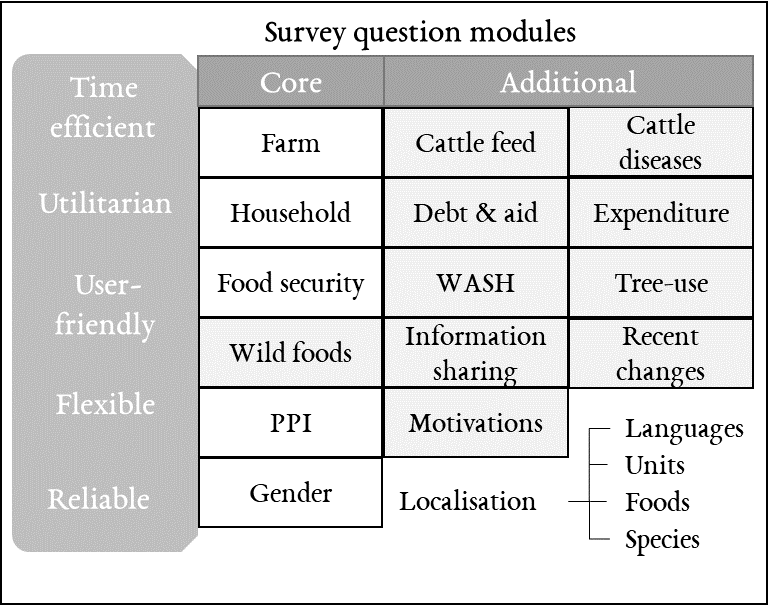
\includegraphics[width=0.6\textwidth]{figs_02/RHOMIS_principlesMods.png}
  \captionsetup{singlelinecheck = false, justification=justified} %left justify caption
  \caption{Core and additional indicators in the RHOMIS tool.Including the progress out of poverty index (PPI) and; water, sanitation and health (WASH) modules from the rural household multi-indicator survey}
  \label{fig:02_1}
\end{figure}

\subsection{Site selection and survey implementation}
Surveys were carried out in two contrasting sites: Trifinio border region of El Salvador, Guatemala and Honduras in Central America, and the Lushoto district in Tanzania, East Africa. Agriculture and livelihoods in both sites are vulnerable to climate change. The contrasting nature of the sites aims to demonstrate the wide applicability of the RHOMIS tool. The sites were selected because they are part of a concerted data gathering effort by various ongoing research programs and projects mentioned below. Lushoto is part of the Eastern Arc Mountains of East Africa which is seen as a global hotspot for biodiversity with diverse micro eco-zones within a relatively small area; mixed crop-livestock, quite intensive farming systems in higher elevation and agro-pastoral farming systems in lower elevation. The Usambara Mountains are an important source of water for north-eastern Tanzania and the Pangani River is utilised for urban water supply, irrigation and hydropower generation. Deforestation, poor land management and inadequate funds for watershed management pose a threat to the long-term supply of quality water from the Usambaras to downstream communities. The supply of water might be further affected by climate change with rainfall predicted to become more irregularly distributed. The agricultural system in the Trifinio region in Central America is dominated by dry, steep and with sporadic rainfall and little to no irrigation infrastructure, where the major crops are maize and beans. Trifinio is part of the `dry corridor' of Central America, and during the past few years rains have become more sporadic, leading to drought conditions since 2014.

In Lushoto, Tanzania, the survey was conducted on a resample of the farm households that were also surveyed in 2012 with the CCAFS research program (https://ccafs.cgiar.org/). In the 2012 survey 200 farm households were randomly selected within the 10 by 10 km land block containing representative agroecologies in the study region that were chosen through a participatory process involving a wide range of partners and expert opinion (\citealp{Kristjanson2012381}; \citealp{Förch2014}). Twenty villages within each block, and then 10 households on average within each village were randomly chosen (\citealp{Kristjanson2012381}) for the household survey. In June 2015 150 households were randomly chosen from the 200 sampled in 2012, and they were interviewed in the first two weeks of July using the digital version of the RHOMIS survey tool. In Trifinio the survey was carried out in conjunction with the baseline survey for the USAID-funded Prueba3 project, implemented by Bioversity, CATIE and Zamorano in Trifinio to test Crowdsourcing Crop Improvement (\citealp{VanEtten2011102}). Villages were selected by collaborating organisations as candidate villages for a bean variety introduction experiment, and a subset of 285 households was randomly selected for the RHOMIS survey from the full list of households taking part in the project. Surveys were trialled with scientific experts in each study region; with scientific and technical staff resident in each study site; with the enumerators who would implement the surveys; and finally with rural households within the intended implementation area of the surveys. Specific changes were made on the phrasing and use of language, on local units of measurement used, on examples of locally available foodstuffs and other products (e.g. types of fertiliser), on the crops, livestock and livestock products commonly produced, routes to market, and common sources of off-farm income. The survey was conducted in Spanish in Trifinio, and in Swahili in Lushoto.

%%%%%%%%%%%%%%%%%%%%%%%%%%%%%%%%%%%%%%%%%%%%%%%%%%%%%%%%%%%%%%%%%%%%%%%%
\section{Results}
%%%%%%%%%%%%%%%%%%%%%%%%%%%%%%%%%%%%%%%%%%%%%%%%%%%%%%%%%%%%%%%%%%%%%%%%

%%%%%%%%%%%%%%%%%%%%%%%%%%%%%%%%%%%%%%%%%%%%%%%%%%%%%%%%%%%%%%%%%%%%%%%%
Across both sites, the running time for the survey was 40–60 minutes per household (Table \ref{tab:02_1}). Gathering data for the food availability indicator took the longest, between 15 and 35 minutes, as it is based on the whole of agricultural production, sales and off farm income. The dietary diversity indicator took the second longest to complete, at around 10 minutes per household, due to the complexity of explaining the different food types, and introducing the concepts of the `flush period' and `lean period'. All other indicators only took up to 5 minutes each (Table \ref{tab:02_1}). The indicators were calculated successfully for most households, we were only unable to calculate \textless1\% of all potential indicator data points due to lack of adequate responses.

The interviewers were asked to rate the `easiness' of gathering the data at the end of each module, whilst undertaking the surveys. Ease related to both the ease of asking and phrasing questions, and the ease of extracting the right type of response from the informant. All modules were rated as `easy' between 50 and 60\% of the time, and rated as medium approximately 30\% of the time, except for off-farm incomes, which was rated `medium' more often than it was rated `easy'. The Progress out of Poverty Indicator was rated as difficult only 5\% of the time, and other modules rated as difficult 11–13\% of the time (details shown in Table \ref{tab:02_1}). This provides evidence that the survey is indeed user friendly. Adaptation of the survey questions, language and training of interviewers took about two weeks in both Trifinio and Lushoto. In Lushoto, Tanzania, in two weeks of data collection with 3 interviewers the responses from 150 households were collected, at a total cost of around US\$5000, including the purchase of three tablets. The implementation in Trifinio was a little more complex, as the RHOMIS survey was only one of two surveys implemented as part of a larger project, so it is not possible to determine survey costs working only with RHOMIS. It does however illustrate that the tool is flexible enough to be used in conjunction with other research methods.

%Field costs for the original WEAI pilots (including enumerator training, translation, and data entry) were $38,000 in Bangladesh (450 households), $56,000 in Guatemala (350 households), and $36,000 in Uganda(367households). The second WEAI pilot costs ranged from $44,000 to $84,000 in Bangladesh and Uganda.
%http://ebrary.ifpri.org/utils/getfile/collection/p15738coll2/id/129719/filename/129930.pdf

\begin{table}[H]
   \caption{
    Time taken to gather data for each indicator, and the ease of that data gathering, as rated by the interviewers during the Lushoto survey, n = 151
  }
  \label{tab:02_1}
  \small
  %\centering
  \captionsetup{singlelinecheck = false, justification=justified} %left justify caption
  \begin{tabular}{l c c c c}  %{p{2cm}p{3cm}p{3cm}p{3cm}p{3cm}}
    \toprule
    Module      & \multirow{2}{3.3cm}{Duration (minutes per household)}  & \multicolumn{3}{c}{Perceived ease of enumerating (\%)}\\ %multirow spreads content over 3cm
    \cmidrule{3-5}
     &   & Easy  & Medium & Difficult \\
    \midrule
      FA          &15-35 &56 &31 &13\\
      HFIAS           &5 &54 &34 &12\\
      Dietary Diversity         & 10 &54 &34 &12\\
      PPI        &3-5 &61 &34 &5\\
      Gender Equity           &5 &61 &28 &11\\
      GHG Emissions         &5 &57 &32 &11\\

    \bottomrule
  \end{tabular}
\end{table}

%%%%%%%%%%%%%%%%%%%%%%%%%%%%%%%%%%%%%%%%%%%%%%%%%%%%%%%%%%%%%%%%%%%%%%%%
\section{Discussion}
%%%%%%%%%%%%%%%%%%%%%%%%%%%%%%%%%%%%%%%%%%%%%%%%%%%%%%%%%%%%%%%%%%%%%%%%

In both study sites the RHOMIS tool met our stated goals of providing rapid, user friendly, and flexible output; both in terms of ease of implementation of the survey by enumerators and by providing efficient data management and analysis. Some of the indicators could be improved upon to give more nuanced interpretations, although there is always tension between speed of survey and detail of results (e.g. \citealp{Mina2008}; \citealp{Coates2013188}; \citealp{DeWeerdt201536}). When considering food security and nutrition there is a clear trade-off between the level of detail that can be achieved in quantifying intake of different foodstuffs of individual actors, versus the goal of obtaining a sufficiently accurate picture of the village or local eating habits (\citealp{Kennedy2011}). In nutrition oriented research the gold standard is (at the moment) the 24 hour recall collecting detailed information on what several individual members of a household consumed the previous 24 h (\citealp{Coates2013188}). However, these data are more time consuming to collect, plus provides only a current snapshot of the nutritional situation. Several surveys per year are required to capture seasonal variation and repeat surveys to measure trends have to take place during the same season to avoid confounding effects. Our approach of asking about frequency of consumption (daily/weekly/monthly) in the `flush' and `lean' periods may be less accurate, but may obtain a general picture much more quickly.

\section{Acknowledgements}
We thank all the people involved in collecting the field data that formed the basis for the analyses and especially the farmers for sharing their valuable information and time. We thank the two anonymous referees and the editors of Agricultural Systems for their useful comments that helped improve this manuscript.
